\begin{post}
	\postdata{Finally mobile}{2011}{9}{26}{21}{19}{5}
	\begin{content}
As pathetic as it might sound, in a country with mobile phone penetration of almost 99\%, until today, I was offline. Well, I had my EU phone, which perfectly works here (it's a Samsung, btw.), but roaming is quite expensive for everyday use, so I wanted to get a Korean phone. Before coming here, my good friend Roman gave me the phone he used while he was on exchange here, so I just needed to get it registered on my Alien ID. Therefore, when our uni arranged some phones for us, I politely declined the offer, thinking that I will simply register the phone I already had.

Now you might think \textit{"Registered? What do you mean?"} or simply \textit{"WTF, dude?"}, but bureaucracy rules Korea, and \textbf{every} Korean phone needs to be registered with their Ministry of Telecommunications or something like that. And registered means that the S/N of the phone is paired with the SSN of the owner. Do you also feel a little bit of 1984? Because of that, some phones do not even have SIM cards, but function merely on this registration basis with regular pre-paid plan.

Unfortunately, Roman forgot to deregister his phone before leaving Korea. And since his Alien ID has already expired, the phone is basically a useless piece of ancient electronics unless he comes here and deregisters it.

Since everything is easier when you speak Korean, I took my buddy Hojoong with me and went phoneshopping. Despite his negotiation efforts, all the offers were too expensive for me. I really don't need to buy another phone, {\H 감사합니다} (\textit{kamsahamnida}). Fortunately, thanks to Jin from the KBS International Center, I managed to contact the company that gave other students the phone deal (which is much cheaper, since they only rent the phone instead of buying it) and today, their guy came to KAIST and handed me my brand new Korean phone. Awesome!

\begin{wrapfigure}{r}{0.5\textwidth}
\centering\fbox{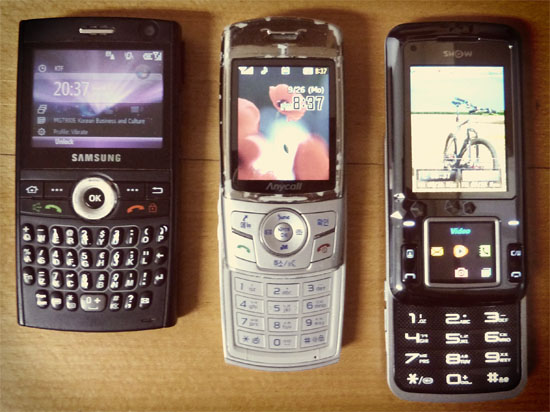
\includegraphics[width=0.5\textwidth]{photos/09/26/phones.jpg}}
\caption{My collection of Korean phones --- Samsung SGH-i600, Anycall (Samsung) SCH-C320, Ever EV-W540}
\end{wrapfigure}The phone is quite cool actually. It is a Ever (KT Tech) EV-W450 phone, that is manufactured exclusively for KT Telecom (hence, KT Tech). It is a "slider", which is currently the most popular kind of phone, apart from touchscreen smartphones, and it is a regular featurephone, so it has Bluetooth and other useful thingies, however, it lacks WiFi or other internet connectivity. And it has, wait for it, Mobile TV a.k.a. DMB! I can watch gameshows and soap operas 24/7, for free! Frankly, I think I won't use it even once, but whatever. Who can say he has a TV in his phone, right:)
	\end{content}
\end{post}
